%!TEX root = poster.tex

\usepackage{tikz}
\usepackage{xcolor}
\usepackage{gensymb}

\usetikzlibrary{shapes, backgrounds, fit, calc, positioning, arrows.meta, bending}

% colorbrewer colours, taken from https://github.com/vtraag/tikz-colorbrewer/blob/master/colorbrewer.sty because I couldn't get \usetikzlibrary{colorbrewer} to work
\definecolor{RdYlBu-4-1}{RGB}{215,25,28}
\definecolor{RdYlBu-4-2}{RGB}{253,174,97}
\definecolor{RdYlBu-4-3}{RGB}{171,217,233}
\definecolor{RdYlBu-4-4}{RGB}{44,123,182}
\definecolor{Blues-4-1}{RGB}{239,243,255}
\definecolor{Blues-4-2}{RGB}{189,215,231}
\definecolor{Blues-4-3}{RGB}{107,174,214}
\definecolor{Blues-4-4}{RGB}{33,113,181}
\definecolor{Oranges-4-1}{RGB}{254,237,222}
\definecolor{Oranges-4-2}{RGB}{253,190,133}
\definecolor{Oranges-4-3}{RGB}{253,141,60}
\definecolor{Oranges-4-4}{RGB}{217,71,1}
\definecolor{Purples-4-1}{RGB}{242,240,247}
\definecolor{Purples-4-2}{RGB}{203,201,226}
\definecolor{Purples-4-3}{RGB}{158,154,200}
\definecolor{Purples-4-4}{RGB}{106,81,163}

\newcommand{\AxisRotator}[1][rotate=0]{%
    \tikz [x=1.1mm,y=1.1mm,line width=.1ex,>={Latex[length=.3em, bend]},#1] \draw (0,0) arc (-150:170:1);%
}

% https://tex.stackexchange.com/a/66220
\def\centerarc[#1](#2)(#3:#4:#5)% Syntax: [draw options] (center) (initial angle:final angle:radius)
    { \draw[#1] ($(#2)+({#5*cos(#3)},{#5*sin(#3)})$) arc (#3:#4:#5); }

\tikzset{
    every picture/.append style={x=5mm, y=5mm},
    circ/.style={circle, draw=black, fill=black, minimum size=2.5mm, inner sep=0mm},
    box/.style={rectangle,draw=black,thick, minimum size=5mm},
    object/.style={draw, dotted, inner sep=0.3em, fill=black!3, rounded corners=1mm},
    desc/.style={rectangle},
    sedge/.style={->, >=stealth},
    dedge/.style={<->, >=stealth},
    varname/.style={midway, above, opacity=1},
    mnist1/.pic={
        % images
        \node[inner sep=0] (input) at (0, 0) {
\includegraphics[scale=0.7, trim={3.5mm 3.5mm 3.5mm 3.5mm}, clip]{resources/mnist-32-11.pdf}};
        \node[inner sep=0] (target) at (20.5, 0) {
\includegraphics[scale=0.7, trim={3.5mm 3.5mm 3.5mm 3.5mm}, clip]{resources/mnist-32-11.pdf}};
        \node[inner sep=0] (y0) at (0, -4) {
\includegraphics[scale=0.7, trim={3.5mm 3.5mm 3.5mm 3.5mm}, clip]{resources/mnist-32-0.pdf}};
        \node[inner sep=0] (y1) at (8, -4) {
\includegraphics[scale=0.7, trim={3.5mm 3.5mm 3.5mm 3.5mm}, clip]{resources/mnist-32-1.pdf}};
        \node[inner sep=0] (y2) at (16, -4) {
\includegraphics[scale=0.7, trim={3.5mm 3.5mm 3.5mm 3.5mm}, clip]{resources/mnist-32-2.pdf}};
        \node[inner sep=0] (y10) at (20.5, -4) {
\includegraphics[scale=0.7, trim={3.5mm 3.5mm 3.5mm 3.5mm}, clip]{resources/mnist-32-10.pdf}};

        % feature vectors
        % input fv
        \node (fvinput bottom)[box, scale=0.36, fill=Oranges-4-3] at (4, -0.5) {};
        \node (fvinput) [box, scale=0.36, fill=Blues-4-4] at (4, 0) {};
        \node [box, scale=0.36, fill=Blues-4-4] at (4, 0.5) {};

        \node (fvinput2 bottom)[box, scale=0.36, fill=Oranges-4-3] at (12, -0.5) {};
        \node (fvinput2) [box, scale=0.36, fill=Blues-4-4] at (12, 0) {};
        \node [box, scale=0.36, fill=Blues-4-4] at (12, 0.5) {};
        % fv0
        \node (fv0 top) [box, scale=0.36, fill=Oranges-4-1] at (4, -3.5) {};
        \node (fv0) [box, scale=0.36, fill=Purples-4-1] at (4, -4) {};
        \node [box, scale=0.36, fill=Oranges-4-1] at (4, -4.5) {};
        % fv1
        \node (fv1 top) [box, scale=0.36, fill=Blues-4-3!50!Blues-4-4] at (12, -3.5) {};
        \node (fv1) [box, scale=0.36, fill=Blues-4-3] at (12, -4) {};
        \node [box, scale=0.36, fill=Oranges-4-2] at (12, -4.5) {};

        % bendy connection between fvs
        \draw [sedge, in=200, out=-20] (y0.south east) to (y1.south west);
        \draw [sedge, in=200, out=-20] (y1.south east) to (y2.south west);
        
        % MSEs
        \draw [ultra thick, color=colorTwo] (fvinput bottom) -- (fv0 top) node (mse0) [midway, scale=0.2, fill=white] {MSE};
        \draw [ultra thick, color=colorTwo] (fvinput2 bottom) -- (fv1 top) node (mse1) [midway, scale=0.2, fill=white] {MSE};

        % input encoder
        \draw [sedge] (input) -- (fvinput) node [midway, scale=0.2, trapezium, rotate=-90, trapezium angle=70, inner ysep=12mm, draw, fill=colorThree!10!white] {Encoder};
        % y0 encoder
        \draw [sedge] (y0) -- (fv0) node [midway, scale=0.2, trapezium, rotate=-90, trapezium angle=70, inner ysep=12mm, draw, fill=colorThree!10!white] {Encoder};
        % y1 encoder
        \draw [sedge] (y1) -- (fv1) node [midway, scale=0.2, trapezium, rotate=-90, trapezium angle=70, inner ysep=12mm, draw, fill=colorThree!10!white] {Encoder};

        % backprop
        \draw [sedge, color=colorTwo] (mse0) -- (y1.north west)
        node [midway, scale=0.2, sloped, above] {$- \partial \text{ MSE}$}
        node [midway, scale=0.2, sloped, below] {$\partial \text{ Step 0}$};
        \draw [sedge, color=colorTwo] (mse1) -- (y2.north west)
        node [midway, scale=0.2, sloped, above] {$- \partial \text{ MSE}$}
        node [midway, scale=0.2, sloped, below] {$\partial \text{ Step 1}$};

        \node [scale=0.2, below = 0mm of y0] {Step 0};
        \node [scale=0.2, below = 0mm of y1] {Step 1};
        \node [scale=0.2, below = 0mm of y2] {Step 2};                        
        \node [scale=0.2, below = 0mm of y10] {Step 10};
        \node [scale=0.2, above = 0mm of input] {Input};
        \node [scale=0.2, above = 0mm of target] {Target};

        \draw [ultra thick, color=colorThree!50!black] (y10) -- (target) node [midway, fill=white, scale=0.2] {set loss};

        \node [scale=0.4] at ($(y2)!0.5!(y10)$) {\ldots};
    },
    mnist2/.pic = {
        % images
        \node[inner sep=0] (input) at (0, 0) {
\includegraphics[scale=0.7, trim={3.5mm 3.5mm 3.5mm 3.5mm}, clip]{resources/mnist-121-11.pdf}};
        \node[inner sep=0] (target) at (20.5, 0) {
\includegraphics[scale=0.7, trim={3.5mm 3.5mm 3.5mm 3.5mm}, clip]{resources/mnist-121-11.pdf}};
        \node[inner sep=0] (y0) at (0, -4) {
\includegraphics[scale=0.7, trim={3.5mm 3.5mm 3.5mm 3.5mm}, clip]{resources/mnist-121-0.pdf}};
        \node[inner sep=0] (y1) at (8, -4) {
\includegraphics[scale=0.7, trim={3.5mm 3.5mm 3.5mm 3.5mm}, clip]{resources/mnist-121-1.pdf}};
        \node[inner sep=0] (y2) at (16, -4) {
\includegraphics[scale=0.7, trim={3.5mm 3.5mm 3.5mm 3.5mm}, clip]{resources/mnist-121-2.pdf}};
        \node[inner sep=0] (y10) at (20.5, -4) {
\includegraphics[scale=0.7, trim={3.5mm 3.5mm 3.5mm 3.5mm}, clip]{resources/mnist-121-10.pdf}};

        % feature vectors
        % input fv
        \node (fvinput bottom)[box, scale=0.36, fill=Purples-4-3] at (4, -0.5) {};
        \node (fvinput) [box, scale=0.36, fill=Oranges-4-4] at (4, 0) {};
        \node [box, scale=0.36, fill=Oranges-4-3] at (4, 0.5) {};

        \node (fvinput2 bottom)[box, scale=0.36, fill=Purples-4-3] at (12, -0.5) {};
        \node (fvinput2) [box, scale=0.36, fill=Oranges-4-4] at (12, 0) {};
        \node [box, scale=0.36, fill=Oranges-4-3] at (12, 0.5) {};
        % fv0
        \node (fv0 top) [box, scale=0.36, fill=Oranges-4-1] at (4, -3.5) {};
        \node (fv0) [box, scale=0.36, fill=Purples-4-1] at (4, -4) {};
        \node [box, scale=0.36, fill=Oranges-4-1] at (4, -4.5) {};
        % fv1
        \node (fv1 top) [box, scale=0.36, fill=Oranges-4-3] at (12, -3.5) {};
        \node (fv1) [box, scale=0.36, fill=Oranges-4-3] at (12, -4) {};
        \node [box, scale=0.36, fill=Blues-4-2] at (12, -4.5) {};

        % bendy connection between fvs
        \draw [sedge, in=200, out=-20] (y0.south east) to (y1.south west);
        \draw [sedge, in=200, out=-20] (y1.south east) to (y2.south west);
        
        % MSEs
        \draw [ultra thick, color=colorTwo] (fvinput bottom) -- (fv0 top) node (mse0) [midway, scale=0.2, fill=white] {MSE};
        \draw [ultra thick, color=colorTwo] (fvinput2 bottom) -- (fv1 top) node (mse1) [midway, scale=0.2, fill=white] {MSE};

        % input encoder
        \draw [sedge] (input) -- (fvinput) node [midway, scale=0.2, trapezium, rotate=-90, trapezium angle=70, inner ysep=12mm, draw, fill=colorThree!10!white] {Encoder};
        % y0 encoder
        \draw [sedge] (y0) -- (fv0) node [midway, scale=0.2, trapezium, rotate=-90, trapezium angle=70, inner ysep=12mm, draw, fill=colorThree!10!white] {Encoder};
        % y1 encoder
        \draw [sedge] (y1) -- (fv1) node [midway, scale=0.2, trapezium, rotate=-90, trapezium angle=70, inner ysep=12mm, draw, fill=colorThree!10!white] {Encoder};

        % backprop
        \draw [sedge, color=colorTwo] (mse0) -- (y1.north west)
        node [midway, scale=0.2, sloped, above] {$- \partial \text{ MSE}$}
        node [midway, scale=0.2, sloped, below] {$\partial \text{ Step 0}$};
        \draw [sedge, color=colorTwo] (mse1) -- (y2.north west)
        node [midway, scale=0.2, sloped, above] {$- \partial \text{ MSE}$}
        node [midway, scale=0.2, sloped, below] {$\partial \text{ Step 1}$};

        \node [scale=0.2, below = 0mm of y0] {Step 0};
        \node [scale=0.2, below = 0mm of y1] {Step 1};
        \node [scale=0.2, below = 0mm of y2] {Step 2};                        
        \node [scale=0.2, below = 0mm of y10] {Step 10};
        \node [scale=0.2, above = 0mm of input] {Input};
        \node [scale=0.2, above = 0mm of target] {Target};

        \draw [ultra thick, color=colorThree!50!black] (y10) -- (target) node [midway, fill=white, scale=0.2] {set loss};

        \node [scale=0.4] at ($(y2)!0.5!(y10)$) {\ldots};
    },
    clevr1/.pic = {
        % images
        \node[inner sep=0] (input) at (0, 1) {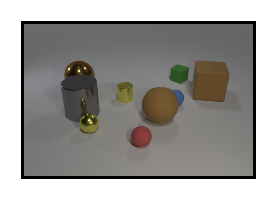
\includegraphics[scale=0.7, trim={3.5mm 3.5mm 3.5mm 3.5mm}, clip]{resources/clevr-23.pdf}};
        \node[inner sep=0] (target) at (18, 1) {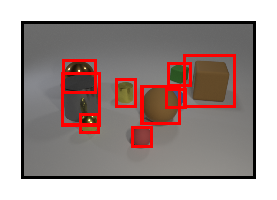
\includegraphics[scale=0.7, trim={3.5mm 3.5mm 3.5mm 3.5mm}, clip]{resources/clevr-23--2.pdf}};
        \node[inner sep=0] (y0) at (0, -4) {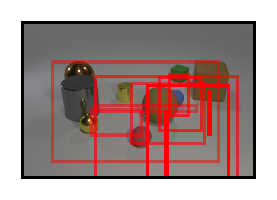
\includegraphics[scale=0.7, trim={3.5mm 3.5mm 3.5mm 3.5mm}, clip]{resources/clevr-23-0.pdf}};
        \node[inner sep=0] (y1) at (11, -4) {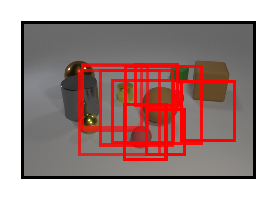
\includegraphics[scale=0.7, trim={3.5mm 3.5mm 3.5mm 3.5mm}, clip]{resources/clevr-23-1.pdf}};
        \node[inner sep=0] (y10) at (18, -4) {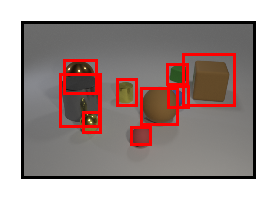
\includegraphics[scale=0.7, trim={3.5mm 3.5mm 3.5mm 3.5mm}, clip]{resources/clevr-23-10.pdf}};

        % feature vectors
        % input fv
        \node (fvinput bottom)[box, scale=0.36, fill=Purples-4-4] at (6, 0.5) {};
        \node (fvinput) [box, scale=0.36, fill=Blues-4-4] at (6, 1) {};
        \node (fvinput top) [box, scale=0.36, fill=Oranges-4-3] at (6, 1.5) {};
        \node [above = 0mm of fvinput top, scale=0.2] {512d};

        \node (fvtarget bottom)[box, scale=0.36, fill=Purples-4-4] at (11, 0.5) {};
        \node (fvtarget) [box, scale=0.36, fill=Blues-4-4] at (11, 1) {};
        \node [box, scale=0.36, fill=Oranges-4-3] at (11, 1.5) {};
        % fv0
        \node (fv0 top) [box, scale=0.36, fill=Oranges-4-1] at (6, -3.5) {};
        \node (fv0) [box, scale=0.36, fill=Blues-4-1] at (6, -4) {};
        \node [box, scale=0.36, fill=Purples-4-1] at (6, -4.5) {};

        % bendy connection between fvs
        \draw [sedge, in=200, out=-20] (y0.south east) to (y1.south west);

        % MSEs
        \draw [ultra thick, color=colorTwo] (fvinput bottom) -- (fv0 top) node (mse0) [midway, scale=0.2, fill=white] {MSE};
        \draw [ultra thick, color=colorThree!50!black] (fvtarget) -- (fvinput) node [midway, scale=0.2, fill=white] {MSE loss};

        % input encoder
        \draw [sedge] (input) -- (fvinput) node [midway, scale=0.2, trapezium, rotate=-90, trapezium angle=70, inner ysep=22mm, draw, fill=colorThree!10!white] {\LARGE ResNet34};
        % y0 encoder
        \draw [sedge] (y0) -- (fv0) node [midway, scale=0.2, trapezium, rotate=-90, trapezium angle=70, inner ysep=12mm, draw, fill=colorThree!10!white] {Encoder};
        % target encoder
        \draw [sedge] (target) -- (fvtarget) node [midway, scale=0.2, trapezium, rotate=90, trapezium angle=70, inner ysep=12mm, draw, fill=colorThree!10!white] {Encoder};

        % backprop
        \draw [sedge, color=colorTwo] (mse0) -- (y1.north west)
        node [midway, scale=0.2, sloped, above] {$- \partial \text{ MSE}$}
        node [midway, scale=0.2, sloped, below] {$\partial \text{ Step 0}$};

        \node [scale=0.2, below = 0mm of y0] {Step 0};
        \node [scale=0.2, below = 0mm of y1] {Step 1};
        \node [scale=0.2, below = 0mm of y10] {Step 10};
        \node [scale=0.2, above = 0mm of input] {Input};
        \node [scale=0.2, above = 0mm of target] {Target};

        \draw [ultra thick, color=colorThree!50!black] (y10) -- (target) node [midway, fill=white, scale=0.2] {set loss};

        \node [scale=0.4] at ($(y1)!0.5!(y10)$) {\ldots};
    },
    symmetry/.pic = {
        % \node [scale=0.9] at (6.5, 2) {The Responsibility Problem};

        \pic at (0, 0) {square};
        \begin{scope}[on background layer]
            \node (s1) [object, fit=(a) (b) (c) (d)] {};
        \end{scope}

        \pic at (13, 0) {square};
        \begin{scope}[on background layer]
            \node (s4) [object, fit=(a) (b) (c) (d)] {};
        \end{scope}

        \pic [rotate=-30] at (4, -3) {square};
        \begin{scope}[on background layer]
            \node (s2) [object, fit=(a) (b) (c) (d)] {};
        \end{scope}

        \pic [rotate=-30+90] at (9, -3) {square};
        \begin{scope}[on background layer]
            \node (s3) [object, fit=(a) (b) (c) (d)] {};
        \end{scope}

        \node [above = 0mm of s1, scale=0.7, color=colorTwo] {(a)};
        \node [above = 0mm of s2, scale=0.7, color=colorTwo] {(c)};
        \node [above = 0mm of s3, scale=0.7, color=colorTwo] {(d)};
        \node [above = 0mm of s4, scale=0.7, color=colorTwo] {(b)};

        \draw [sedge] (s1) -- (s4) node [above, midway] {\raisebox{-0.3mm}{\AxisRotator[xscale=-1]} $90\degree$};
        \draw [sedge, draw=red] (s2) -- (s3) node [below, midway] {\raisebox{-0.5mm}{\AxisRotator[xscale=-1]} $\epsilon$} node [above, midway, red, scale=0.4] {discontinuity};
        \draw [sedge] (s1.south) to[bend right] node [below=1.5mm, midway] {\raisebox{-0.5mm}{\AxisRotator[xscale=-1]} $30\degree$} (s2.west);
        \draw [sedge, text width=1.8cm] (s3.east) to[bend right] node [below=4.5mm, pos=0.8] {\raisebox{-0.5mm}{\AxisRotator[xscale=-1]} $60\degree - \epsilon$} (s4.south);
    },
    square/.pic = {
        \node (a) [circ, fill=RdYlBu-4-1] at (-0.8, 0.8) {};
        \node (b) [circ, fill=RdYlBu-4-2] at (0.8, 0.8) {};
        \node (c) [circ, fill=RdYlBu-4-3] at (0.8, -0.8) {};
        \node (d) [circ, fill=RdYlBu-4-4] at (-0.8, -0.8) {};
    },
    square2/.pic = {
        \node (a) [circ, fill=colorOne] at (-0.8, 0.8) {};
        \node (b) [circ, fill=colorOne] at (0.8, 0.8) {};
        \node (c) [circ, fill=colorOne] at (0.8, -0.8) {};
        \node (d) [circ, fill=colorOne] at (-0.8, -0.8) {};
    },
    model/.pic = {
        \pic (inputs) at (0, 0) {inputs};
        \pic (sort) at (8, 0) {sorted};
        \pic [scale=1.25, every node/.style={transform shape}] (output) at (12.75, 0) {output};
        \pic (dweights) at (16, 0) {dweights};
        \pic (cweights) at (20.5, 0) {cweights};

        \node at (2.5, 1.5) {$\mX$};

        \node at (6.35, -1.2) {\scriptsize sort};
        \draw [sedge] (5.6,  0.0) -- (7.2,  0.0);
        \draw [sedge] (5.6,  0.7) -- (7.2,  0.7);
        \draw [sedge] (5.6, -0.7) -- (7.2, -0.7);

        \node at (8.75, 1.5) {$\mvX$};

        \draw [sedge] (10.2,  0.0) -- (12,  0.0);
        \draw [sedge] (10.2,  0.7) -- (12,  0.7);
        \draw [sedge] (10.2, -0.7) -- (12, -0.7);

        \node at (12.75, 1.4) {$\vy$};
        \node at (12.75, -1.35) {\scriptsize dot product};

        \draw [sedge] (15.2,  0.0) -- (13.5,  0.0);
        \draw [sedge] (15.2,  0.7) -- (13.5,  0.7);
        \draw [sedge] (15.2, -0.7) -- (13.5, -0.7);

        \node at (17.0, 1.4) {\scriptsize $f([\scriptscriptstyle 0, \frac{1}{3}, \frac{2}{3}, 1 \displaystyle], \mbW)$};

        \node at (19.2, -1.2) {\scriptsize discretise};

        \node at (23, 1.4) {\scriptsize $f(\cdot, \mbW)$};

        \draw [sedge] (20,  0.0) -- (18.2,  0.0);
        \draw [sedge] (20,  0.7) -- (18.2,  0.7);
        \draw [sedge] (20, -0.7) -- (18.2, -0.7);
    },
    sorted/.pic = {
        \node [box, scale=0.5, fill=Blues-4-4] at (0.0, 0.7) {};
        \node [box, scale=0.5, fill=Blues-4-3] at (0.5, 0.7) {};
        \node [box, scale=0.5, fill=Blues-4-2] at (1.0, 0.7) {};
        \node [box, scale=0.5, fill=Blues-4-1] at (1.5, 0.7) {};

        \node [box, scale=0.5, fill=Oranges-4-4] at (0.0, 0.0) {};
        \node [box, scale=0.5, fill=Oranges-4-3] at (0.5, 0.0) {};
        \node [box, scale=0.5, fill=Oranges-4-2] at (1.0, 0.0) {};
        \node [box, scale=0.5, fill=Oranges-4-1] at (1.5, 0.0) {};

        \node [box, scale=0.5, fill=Purples-4-4] at (0.0, -0.7) {};
        \node [box, scale=0.5, fill=Purples-4-3] at (0.5, -0.7) {};
        \node [box, scale=0.5, fill=Purples-4-2] at (1.0, -0.7) {};
        \node [box, scale=0.5, fill=Purples-4-1] at (1.5, -0.7) {};
    },
    inputs/.pic = {
        \node at (0, 0) {$\Bigg\{$};
        \node at (5, 0) {$\Bigg\}$};

        \node [box, scale=0.625, fill=Blues-4-3] at (1, 0.625) {};
        \node [box, scale=0.625, fill=Oranges-4-4] at (1, 0.0) {};
        \node [box, scale=0.625, fill=Purples-4-3] at (1, -0.625) {};

        \node [box, scale=0.625, fill=Blues-4-2] at (2, 0.625) {};
        \node [box, scale=0.625, fill=Oranges-4-2] at (2, 0.0) {};
        \node [box, scale=0.625, fill=Purples-4-1] at (2, -0.625) {};

        \node [box, scale=0.625, fill=Blues-4-1] at (3, 0.625) {};
        \node [box, scale=0.625, fill=Oranges-4-3] at (3, 0.0) {};
        \node [box, scale=0.625, fill=Purples-4-4] at (3, -0.625) {};

        \node [box, scale=0.625, fill=Blues-4-4] at (4, 0.625) {};
        \node [box, scale=0.625, fill=Oranges-4-1] at (4, 0.0) {};
        \node [box, scale=0.625, fill=Purples-4-2] at (4, -0.625) {};
    },
    dweights/.pic = {
        \node [box, scale=0.5, fill=Blues-4-3] at (0.0, 0.7) {};
        \node [box, scale=0.5, fill=Blues-4-3] at (0.5, 0.7) {};
        \node [box, scale=0.5, fill=Blues-4-3] at (1.0, 0.7) {};
        \node [box, scale=0.5, fill=Blues-4-3] at (1.5, 0.7) {};

        \node [box, scale=0.5, fill=Oranges-4-2] at (0.0, 0.0) {};
        \node [box, scale=0.5, fill=Oranges-4-3] at (0.5, 0.0) {};
        \node [box, scale=0.5, fill=Oranges-4-3] at (1.0, 0.0) {};
        \node [box, scale=0.5, fill=Oranges-4-2] at (1.5, 0.0) {};

        \node [box, scale=0.5, fill=Purples-4-1] at (0.0, -0.7) {};
        \node [box, scale=0.5, fill=Purples-4-1] at (0.5, -0.7) {};
        \node [box, scale=0.5, fill=Purples-4-3] at (1.0, -0.7) {};
        \node [box, scale=0.5, fill=Purples-4-4] at (1.5, -0.7) {};
    },
    cweights/.pic = {
        \draw [very thick] (0, 0) -- (5, 0);
        \draw [very thick, sedge] (0, -1) -- (0, 1.4);
        \draw [very thick] (5, -1) -- (5, 1.4);

        \draw [thick, draw=Blues-4-3] (0, 0.5) -- (2.5, 0.5) -- (5, 0.5);
        \draw [thick, draw=Oranges-4-3] (0, 0) -- (2.5, 1) -- (5, 0);
        \draw [thick, draw=Purples-4-3] (0, -0.5) -- (2.5, -0.5) -- (5, 1);

        \node [circle, scale=0.25, fill=Oranges-4-4] at (0, 0) {};
        \node [circle, scale=0.25, fill=Blues-4-4] at (0, 0.5) {};
        \node [circle, scale=0.25, fill=Purples-4-4] at (0, -0.5) {};
        \node [circle, scale=0.25, fill=Oranges-4-4] at (1.667, 0.666) {};
        \node [circle, scale=0.25, fill=Blues-4-4] at (1.667, 0.5) {};
        \node [circle, scale=0.25, fill=Purples-4-4] at (1.667, -0.5) {};
        \node [circle, scale=0.25, fill=Oranges-4-4] at (3.333, 0.666) {};
        \node [circle, scale=0.25, fill=Blues-4-4] at (3.333, 0.5) {};
        \node [circle, scale=0.25, fill=Purples-4-4] at (3.333, 0) {};
        \node [circle, scale=0.25, fill=Purples-4-4] at (5, 1) {};
        \node [circle, scale=0.25, fill=Blues-4-4] at (5, 0.5) {};
        \node [circle, scale=0.25, fill=Oranges-4-4] at (5, 0) {};
    },
    output/.pic = {
        \node [box, scale=0.5, fill=Blues-4-3!50!Blues-4-2] at (0, 0.5) {};
        \node [box, scale=0.5, fill=Oranges-4-3!50!Oranges-4-2] at (0, 0.0) {};
        \node [box, scale=0.5, fill=Purples-4-1] at (0, -0.5) {};
    },
    ae/.pic = {
        \pic at (-3, 0) {square2};
        \begin{scope}[on background layer]
            \node (s1) [object, fit=(a) (b) (c) (d)] {};
        \end{scope}

        \node (enc) [trapezium, draw, rotate=-90, inner ysep=3.5mm, trapezium angle=70, fill=colorThree!10] at (3.5, 0) {Encoder};
        \node [box, scale=0.5, fill=Blues-4-3] at (5.5, 0.5) {};
        \node (fv) [box, scale=0.5, fill=Oranges-4-3] at (5.5, 0) {};
        \node [box, scale=0.5, fill=Purples-4-3] at (5.5, -0.5) {};
        \node (dec) [trapezium, draw, rotate=90, inner ysep=3.5mm, trapezium angle=70, fill=colorThree!10] at (7.5, 0) {~~~~MLP~~~~};


        \node [color=colorOne] (i4) at (0,  1.5) {(-1, -1)};
        \node [color=colorOne] (i3) at (0,  0.5) {(~1, -1)};
        \node [color=colorOne] (i2) at (0, -0.5) {(~1, ~1)};
        \node [color=colorOne] (i1) at (0, -1.5) {(-1, ~1)};

        \node [color=RdYlBu-4-1] (o4) at (11,  1.5) {(-1, ~1)};
        \node [color=RdYlBu-4-2] (o3) at (11,  0.5) {(~1, ~1)};
        \node [color=RdYlBu-4-3] (o2) at (11, -0.5) {(~1, -1)};
        \node [color=RdYlBu-4-4] (o1) at (11, -1.5) {(-1, -1)};

        \pic at (14, 0) {square};
        \begin{scope}[on background layer]
            \node (s2) [object, fit=(a) (b) (c) (d)] {};
        \end{scope}


        \draw [sedge] (i1) -- (enc.south |- i1);
        \draw [sedge] (i2) -- (enc.south |- i2);
        \draw [sedge] (i3) -- (enc.south |- i3);
        \draw [sedge] (i4) -- (enc.south |- i4);
        \draw [sedge] (enc) -- (fv);
        \draw [sedge] (fv) -- (dec);
        \draw [sedge] (dec.south |- o1) -- (o1);
        \draw [sedge] (dec.south |- o2) -- (o2);
        \draw [sedge] (dec.south |- o3) -- (o3);
        \draw [sedge] (dec.south |- o4) -- (o4);

    }
}
